%!TEX root = ../project.tex
\part{Analysis}

%%%
\section{Investigation}

%%
\subsection{Problem}
Dr.~Naylor, who teaches astronomy, needs a way to help his students visualise
the orbits of the planets to help them to understand Kepler's laws of planetary
motion.

%%
\subsection{Current Solution}
\begin{figure}[h]
	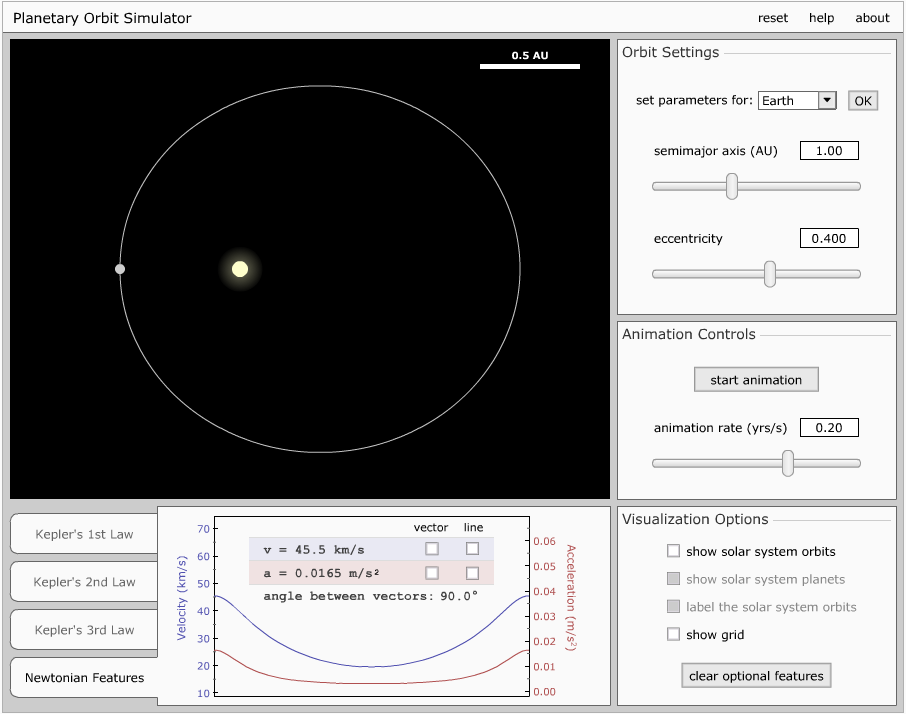
\includegraphics[width=\textwidth]{./img/existing-solution.png}
	\caption{Screenshot of the current system}
	\label{fig:existing-solution}
\end{figure}
The current system shows the solar system in 2 dimensions. It only shows one
planet by default but there is the option to show the others. It only allows one
planet's properties to be manipulated at a time, and the properties that can be
changed are the semimajor axis and eccentricity (and these can be set to the
values of a real planet using the drop-down menu). The animation speed can also
be adjusted. The program has strict limits to what values these parameters can
be set to. The strength of this solution is its visualisations of Kepler's laws,
which is what the end user really needs from the program.

%%
\subsection{Prospective Users}
My main user will be Dr.~Naylor, as he is the astronomy teacher at my school. He
would like to be able to stand in front of a class and use the program to help
the students visualise Kepler's laws while he explains them. It may also be
useful if the program can be used by the students in their own time, if they
didn't understand something in the lesson. I would also like to allow the
student to experiment with as I think it would make them more interested.
Dr.~Naylor isn't very computer literate, so the interface should be easy to
understand. Also if I'm aiming to have the students use it do there will be a
wide variety of abilities. 

%%
\subsection{User's Needs and Limitations} 
Dr.~Naylor needs a system that will allow him to easily demonstrate Kepler's
laws of planetary motion in front of a class of students. He needs to be able
to change the semimajor axis and eccentricity of a planets orbit, and have
presets for different planets in our solar system. 

%%%
\section{Objectives and Constraints of the New System}


%%%
\section{Potential Solutions}

%%
\subsection{Standalone Client}
This is a standalone application to be installed on the users computer. The
user's data and preferences would all be stored on the host computer. This would
allow the user to use the application without an internet connection, but they
will need permission to install programs to their computer, and it would take up
space on their hard drive. If I choose to do a standalone client I will need to
choose the language it is written in and the graphics library I choose to use.
The languages I am choosing between are C and Common Lisp, and the graphics
libraries are OpenGL and SDL.

\paragraph{C}
Writing the program in C would produce a very fast application however it would
be hard to code. The speed of my application is quite important because it will
be run on the school computers, which are not the fastest. Also C is the native
language for both OpenGL and SDL so they both work very well with it and are
well documented. C is a very popular language so finding answers to any
questions that I might have will be very easy.

\paragraph{Common Lisp} 
Common Lisp allows be to write and debug programs very quickly compared to C,
and good Lisp code can be almost as fast as C. However it will most likely be
slower than the C solution. There are bindings for OpenGL and SDL so I can use
whichever I decide on, but neither have very good documentation. Also, I am well
practised in Lisp at the moment than I am with C.

\paragraph{OpenGL}

\paragraph{SDL}

%%
\subsection{Web Based Client}
Another option is an application that runs inside the browser. The advantage of
this is that the user doesn't have to store anything on their own computer, and
it would be easier for the students to use. However I don't know any languages
that would allow me to do this, so I would have to learn a new one. The best
option for me would be Clojure, as it is a Lisp dialect that compiles to
Javascript. This shouldn't be too hard for me to learn as I already use another
Lisp dialect. If I decide to use 3D graphics a web based client would not be as
good as it would run very slowly. Also I would have to worry about my program
being compatible with different browsers as well as different operating systems
but it should be very easy to make it work on any platform. 
